\section{Basic Features}

\begin{frame}[fragile]
    \frametitle{Data Types (1)}

    \begin{itemize}
        \item Scalars
        \begin{itemize}
            \item Integers: \texttt{u32, i64, usize, \dots}
            \item Floats: \texttt{f32, f64}
            \item Boolean: \texttt{bool}
            \item Character: \texttt{char}
        \end{itemize}
        \item Structs
    \begin{lstlisting}[language=rust]
struct Foo {
    field1: u32,
    field2: String,
}
    \end{lstlisting}
    \end{itemize}
\end{frame}

\begin{frame}[fragile]
    \frametitle{Data Types (2)}

    \begin{itemize}
        \item Tuples
    \begin{lstlisting}[language=rust]
let mut tuple = (1, "foo", 42);     // tuple length is fixed
tuple.0 += 1;                       // values are mutable
let (x, y, z) = tuple;              // destructuring
    \end{lstlisting}
        \item Arrays
    \begin{lstlisting}[language=rust]
let mut array: [u32; 2] = [1, 2];   // arrays have a fixed size
array[3] += 1;                      // runtime error (bounds checked)
let foo = [0; 12];                  // array with 12 elements with value 0
    \end{lstlisting}
    \end{itemize}
\end{frame}

\begin{frame}[fragile]
    \frametitle{Strings and Slices}

    \begin{columns}
    \begin{column}{0.5\textwidth}

    \begin{overlayarea}{\linewidth}{7cm}
    \begin{onlyenv}<1->
    \begin{lstlisting}[language=rust]
    let s = String::from("hello world");
    // String ~= Vec<char>
    let world = &s[6..11];
    // &str ~= &[char]
    \end{lstlisting}
    \end{onlyenv}

    \begin{onlyenv}<2->
    \begin{lstlisting}[language=rust]
    &s[0..11]   // = "hello world"
    &s[6..]     // = "world"
    &s[..5]     // = "hello"
    &s[..]      // = "hello world"
    \end{lstlisting}
    \end{onlyenv}

    \begin{onlyenv}<3->
    \begin{lstlisting}[language=rust]
    let a = [1, 2, 3];
    &a[0..1]    // = [1]
    \end{lstlisting}
    \end{onlyenv}

    \end{overlayarea}
    \end{column}

    \begin{column}{0.5\textwidth}
        \begin{figure}
            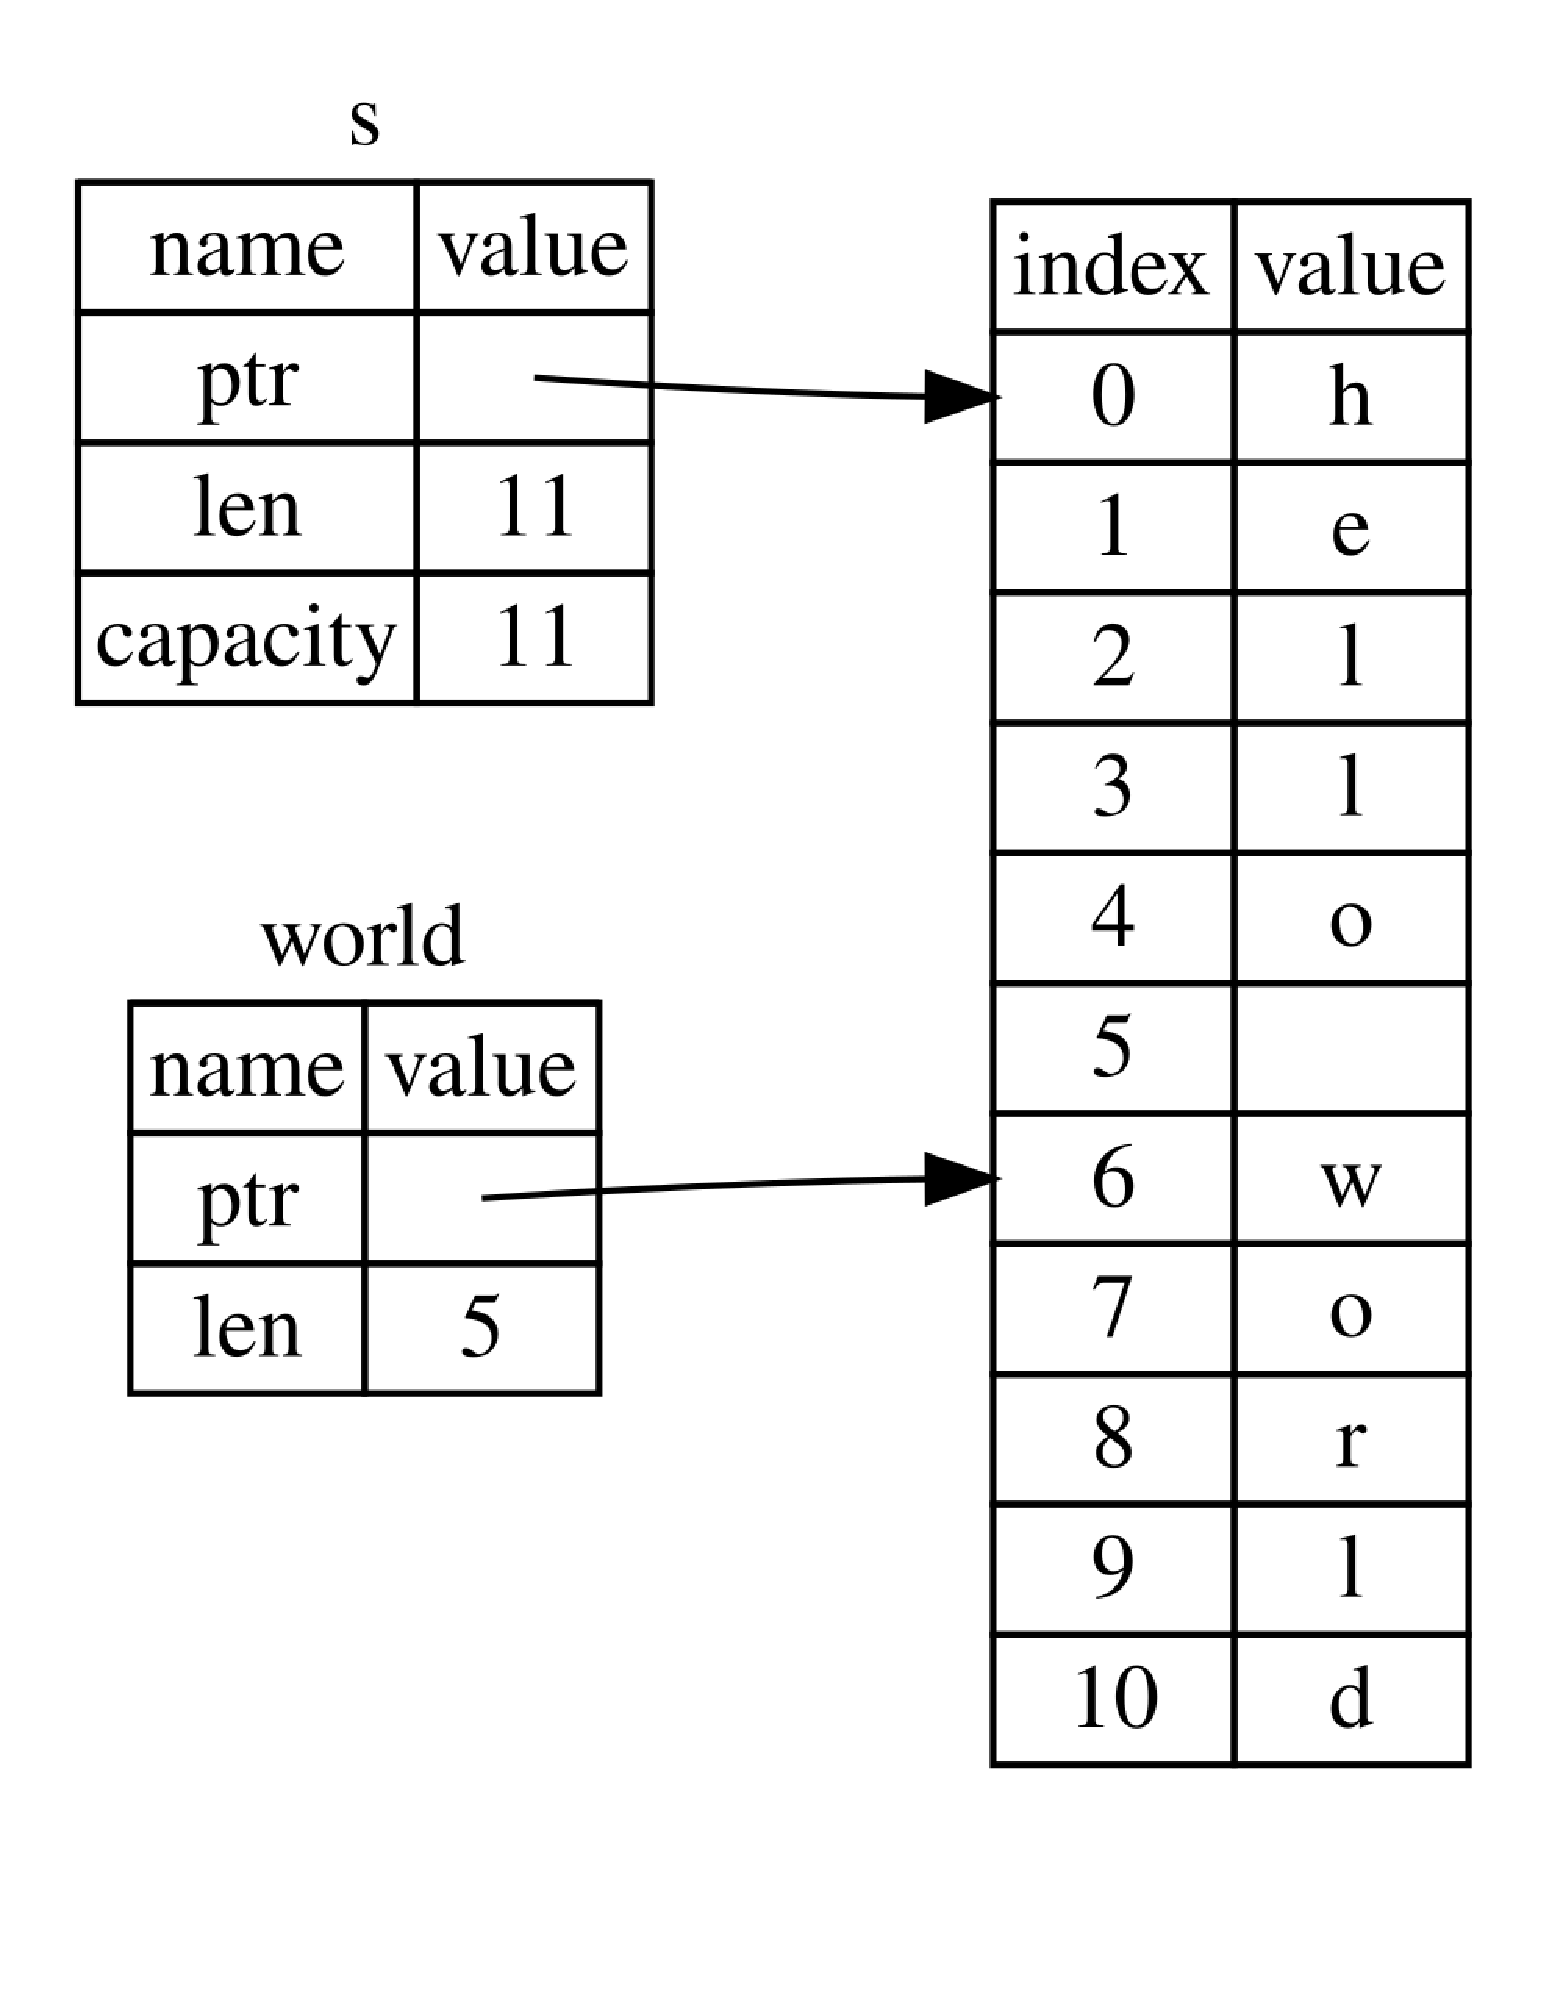
\includegraphics[width=.7\textwidth]{img/string-slice.pdf}
        \end{figure}
    \end{column}
    \end{columns}
\end{frame}

\begin{frame}[fragile]
    \frametitle{Control Structures}

    \begin{itemize}
        \item If expressions
    \begin{lstlisting}[language=rust]
if condition { println!("foo"); } else { println!("bar"); }
let val = if condition { 4 } else { 5 };
    \end{lstlisting}
        \item Loop
    \begin{lstlisting}[language=rust]
loop { }
    \end{lstlisting}
        \item While
    \begin{lstlisting}[language=rust]
while condition { }
    \end{lstlisting}
        \item For
    \begin{lstlisting}[language=rust]
for i in 0..10 { }
    \end{lstlisting}
    \end{itemize}
\end{frame}

\begin{frame}[fragile]
    \frametitle{Exercise 1 -- String Operations}

    \begin{itemize}
        \item Clone the repository:
    \begin{lstlisting}[language=bash]
$ git clone https://...
    \end{lstlisting}
        \item First exercise is in directory ``words''
        \item Fill in the implementation of the functions
        \item Use the existing tests to verify your implementation:
    \begin{lstlisting}[language=bash]
$ cargo test
    \end{lstlisting}
        \item Hint: use the standard library (\url{https://doc.rust-lang.org/stable}):
        \begin{itemize}
            \item \texttt{str::chars}
            \item \texttt{char::is\_uppercase}
            \item \texttt{str::split\_whitespace}
        \end{itemize}
    \end{itemize}
\end{frame}
